\documentclass[a4paper, 12pt]{article}
%\documentclass{book}

% Important Packages:
 \usepackage{amsmath}    % need for subequations
 \usepackage{amsfonts}
 \usepackage{amsthm}
 \usepackage{graphicx}   % need for figures
 \usepackage{verbatim}   % useful for program listings
 \usepackage{tikz,tkz-euclide}
 \usepackage{amssymb}
 
 \usetikzlibrary{calc,patterns,angles,quotes}
\usetkzobj{all}

\def\deg{^{\circ}}
\newcommand\heading[1]{\ \\\large{\textbf{#1}}}
\newcommand\ora[1]{\overrightarrow{#1}}

\def\thm{Th\textsuperscript{\underline{m}}}

%------------------end---preamble--------------------
 
 % Useful macros 
 \def\tcb#1{\color{blue}{#1}}
 \def\tcr#1{\color{red}{#1}}	
 \def\tcg#1{\color{green}{#1}}
 \def\be{\begin{eqnarray}}	 	\def\ee{\end{eqnarray}}
 \def\bea{\begin{eqnarray}}	 	\def\eea{\end{eqnarray}}
 \def\bean{\begin{eqnarray*}}	\def\eean{\end{eqnarray*}}
 
 \def\D{\displaystyle}
 \def\T{\textstyle}
 \def\l{\left}
 \def\r{\right}
 \def\nf{n_{\!f}} % quark flavours
 \def\pa{\partial}
 \def\eg{e.\,g.}
 \def\ie{i.\,e.}

 \def\be{\begin{equation}}
 \def\ee{\end{equation}}
 \def\bea{\begin{eqnarray}}
 \def\eea{\end{eqnarray}}
 \def\bean{\begin{eqnarray*}}
 \def\eean{\end{eqnarray*}}
 \def\gsim{\mathrel{\rlap{\lower0.2em\hbox{$\sim$}}\raise0.2em\hbox{$>$}}}
 \def\ksim{\mathrel{\rlap{\lower0.2em\hbox{$\sim$}}\raise0.2em\hbox{$<$}}}
 \def\kg{\mathrel{\rlap{\lower0.25em\hbox{$>$}}\raise0.25em\hbox{$<$}}}
 
 \def\AA{${\buildrel_{\circ} \over {\mathrm{A}}}$}
 \def\bm#1{\mbox{\boldmath$#1$}}
 \newcommand{\eq}[1]{(\ref{#1})} 
 \def\pd{\partial}
 \def\d{\textrm{d}} 
 \def\T{\textstyle}
 \def\eg{e.\,g.}	% exempli gratia (for the sake of example)
 \def\ie{i.\,e.}	% id est (that is)


 % Page configuration:
 \topmargin -2.0cm
 \oddsidemargin -0.85cm
 \evensidemargin -0.85cm
 \textwidth 18cm
 \textheight 24cm
 
\begin{document}
\begin{center}
\textbf{April Camp 2019 \\ Senior Test 4} \\
\textbf{Solutions}
\end{center}
\vspace{5mm}

\begin{enumerate}

%  2018 shortlist G2
\item[1.]  \textit{Let $ABC$ be a triangle with $AB = AC$, and let $M$ be the midpoint of $BC$. Let $P$ be a point such that $PB < PC$ and $PA$ is parallel to $BC$. Let $X$ and $Y$ be points on the lines $PB$ and $PC$, respectively, so that $B$ lies on the segment $PX$, $C$ lies on the segment $PY$, and $\angle PXM = \angle PYM$. Prove that the quadrilateral $APXY$ is cyclic.
}
\vspace{5mm}

\textbf{Proof: } Since $AB = AC$, $AM$ is the perpendicular bisector of $BC$, hence $\angle PAM = \angle AMC = 90^\circ$.

% Sketch
\begin{figure}[h]
    \centering
    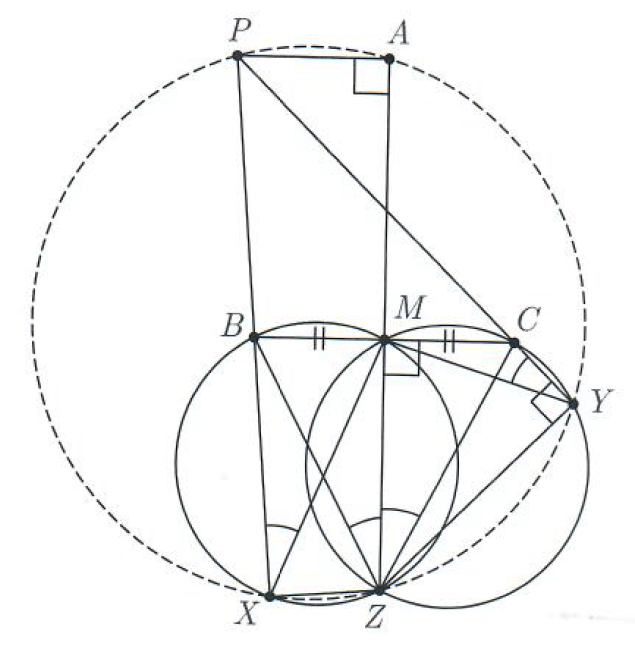
\includegraphics[width = 0.5\textwidth]{2018_G2}
\end{figure}

Now let $Z$ be the common point of $AM$ and the perpendicular through $Y$ to $PC$ (notice that $Z$ lies on to the ray $AM$ beyond $M$). We have $\angle PAZ = \angle PYZ = 90^\circ$. Thus the points $P, A, Y$ and $Z$ are concyclic.

Since $\angle CMZ = \angle CYZ = 90^\circ$, the quadrilateral $CYZM$ is cyclic, hence $\angle CZM = \angle CYM$. By the condition in the statement, $\angle CYM = \angle BXM$, and, by symmetry in $ZM$, $\angle CZM = \angle BZM$. Therefore, $\angle BXM = \angle BZM$. It follows that the points $B, X, Z$, and $M$ are concyclic, hence $\angle BXZ = 180^\circ - \angle BMZ = 90^\circ$.

Finally, we have $\angle PXZ = \angle PYZ = \angle PAZ = 90^\circ$, hence the five points $P, A, X, Y, Z$ are concyclic. In particular, the quadrilateral $APXY$ is cyclic, as required.  \qed \\



\textbf{Comment 1. }  Clearly, the key point $Z$ from the solution above can be introduced in several different ways, e.g. as the second meeting point of the circle $CMY$ and the line $AM$, or as the second meeting point of the circles $CMY$ and $BMX$, etc.

For some definitions of $Z$ its location is not obvious. For instance, if $Z$ is defined as a common point of $AM$ and the perpendicular through $X$ to $PX$, it is not clear that $Z$ lies on the ray $AM$ beyond $M$. To avoid such slippery details some more restrictions on the construction may be required. \\

\textbf{Comment 2. }  Let us discuss a connection to the Miquel point of a cyclic quadrilateral. Set $X' = MX \cap PC$, $Y' = MY \cap PB$, and $Q = XY \cap X'Y'$ (see figure below).

We claim that $BC \parallel PQ$. (One way of proving this is following. Notice that the quadruple of lines $PX$, $PM$, $PY$, $PQ$ is harmonic, hence the quadruple $B, M, C$, $PQ \cap BC$ of their intersection points with $BC$ is harmonic. Since $M$ is the midpoint of $BC$, $PQ \cap BC$ is an ideal point, i.e. $PQ \parallel BC$.)

It follows from the given equality $\angle PXM = \angle PYM$ that the quadrilateral $XYX'Y'$ is cyclic. Note that $A$ is the projection of $M$ onto $PQ$. By a known contradiction, $A$ is the Miquel point for the sidelines $XY$, $XY'$, $X'Y$, $X'Y'$. In particular, the circle $PXY$ passes through $A$.

% Sketch, G2, 2
\begin{figure}[h]
    \centering
    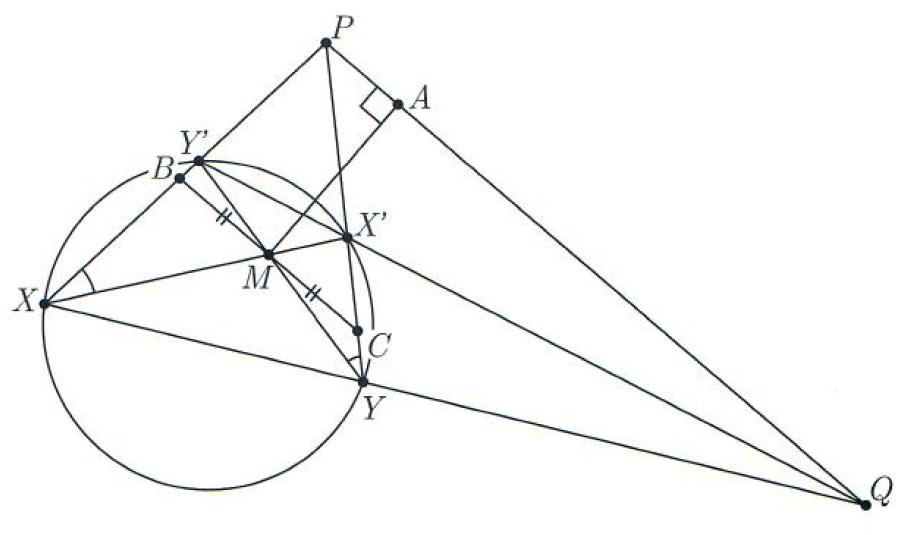
\includegraphics[width=0.6\textwidth]{2018_G2_2}
\end{figure}

\textbf{Comment 3. } An alternative approach is the following. One can note that the (oriented) lengths of the segments $CY$ and $BX$ are both linear functions of a parameter $t = \cot{\angle PXM}$. As $t$ varies, the intersection point $S$ of the perpendicular bisectors of $PX$ and $PY$ traces a fixed line, thus the family of circles $PXY$ has a fixed common point (other than $P$). By checking particular cases, one can show that this fixed point is $A$. \\

\textbf{Comment 4. }  The problem states that $\angle PXM = \angle PYM$ implies that $APXY$ is cyclic. The original submission claims that these two conditions are in fact equivalent. The Problem Selection Committee omitted the converse part since it follows easily from the direct one, by reversing arguments.



% 2018 shortlist C3
\vspace{5mm}
\item[2.]  \textit{Let $n$ be a given positive integer.  Sisyphus performs a sequence of turns on a board consisting of $n+1$ squares in a row, numbered from 0 to $n$ from left to right.  Initially, $n$ stones are put into square 0, and the other squares are empty. At every turn, Sisyphus chooses an nonempty square, say with $k$ stones, takes one of those stones and moves it to the right by at most $k$ squares (the stone should stay within the board). Sisyphus' aim is to move all $n$ stones to square $n$.}

\textit{Prove that Sisyphus cannot reach the aim in less than
 $$\left\lceil \frac{n}{1} \right\rceil + \left\lceil \frac{n}{2} \right\rceil +\left\lceil \frac{n}{3} \right\rceil + \dots + \left\lceil \frac{n}{n} \right\rceil
$$
turns. (As usual, $\lceil x \rceil$ stands for the least integer not smaller than $x$.)
} \\

\textbf{Solution. } The stones are indistinguishable, and all have the same origin and the same final position. So, at any turn we can prescribe which stone from the chosen square to move. We do it in the following manner. Number the stones from $1$ to $n$. At any turn, after choosing a square, Sisyphus moves the stone with the largest number from this square.

This way, when stone $k$ is moved from some square, that square contains not more than $k$ stones (since all their numbers are at most $k$). Therefore, stone $k$ is moved by at most $k$ squares at each turn.  Since the total shift of the stone is exactly $n$, at least $\lceil n/k \rceil$ moves of stone $k$ should have been made, for every $k = 1, 2, \dots, n$.

By summing up over all $k = 1, 2, \dots, n$, we get the required estimate. \qed \\

\textbf{Comment. } The original submission contained the second part, asking for which values of $n$ the equality can be achieved.  The answer is $n = 1, 2, 3, 4, 5, 7$. The Problem Selection Committee considered this part to be less suitable for the competition, due to technicalities.


\vspace{5mm}
\item[3.]  \textit{Four positive integers $x, y, z$, and $t$ satisfy the relations
$$ xy - zt = x + y = z + t. $$
Is it possible that both $xy$ and $zt$ are perfect squares?}
 \vspace{5mm}

\textbf{Answer: } No \\

\textbf{Solution 1. } Arguing indirectly, assume that $xy = a^2$ and $zt = c^2$ with $a, c > 0$.

Suppose that the number $x+y = z+t$ is odd. Then $x$ and $y$ have opposite parity, as well as $z$ and $t$.  This means that both $xy$ and $zt$ are even, as well as $xy - zt = x + y$; a contradiction. Thus $x+y$ is even, so the number $s = \frac{x+y}{2} = \frac{z+t}{2}$ is a positive integer. 

Next, we set $b = \frac{|x-y|}{2}$, $d = \frac{|z-t|}{2}$. Now, the problem conditions yield
\begin{equation} \label{n51}
    s^2 = a^2 + b^2 = c^2 + d^2
\end{equation}
and
\begin{equation} \label{n52}
    2s = a^2 - c^2 = d^2 - b^2
\end{equation}
(the last equality in (\ref{n51}) follows from (\ref{n52})). We readily get from (\ref{n52}) that $a, d, > 0$.

In the sequel we will use only the relations (\ref{n51}) and (\ref{n52}), along with the fact that $a, d, s$ are positive integers, while $b$ and $c$ are nonnegative integers, at most one of which may be zero.  Since both relations are symmetric with respect to the simultaneous swappings $a \leftrightarrow d$ and $b \leftrightarrow c$, we assume, without loss of generality, that $b \geq c$ (and hence $b > 0$). Therefore, $d^2 = 2s + b^2 > c^2$, whence
\begin{equation} \label{n53}
    d^2 > \frac{c^2 + d^2}{2} = \frac{s^2}{2}.
\end{equation}

On the other hand, since $d^2 - b^2$ is even by (\ref{n52}), the numbers $b$ and $d$ have the same parity, so $0 < b \leq d-2$. Therefore,
\begin{equation} \label{n54}
2s = d^2 - b^2 \geq d^2 - (d-2)^2 = 4(d-1), \qquad \textrm{i.e., } \quad d \leq \frac{s}{2} + 1.
\end{equation}

Combining (\ref{n53}) and (\ref{n54}) we obtain
$$
2s^2 < 4d^2 \leq 4 \left(  \frac{s}{2} + 1 \right)^2, \quad \textrm{or} \quad (s-2)^2 < 8,
$$
which yields $s \leq 4$.

Finally, an easy check shows that each number of the form $s^2$ with $1 \leq s \leq 4$ has a unique representation as a sum of two squares, namely $s^2 = s^2 + 0^2$. Thus, (\ref{n51}) along with $a, d > 0$ imply $b = c = 0$, which is impossible. \qed \\

\textbf{Solution 2. } We start with a complete description of all 4-tuples $(x, y, z, t)$ of positive integers satisfying the given equation.  As in the solution above, we notice that the numbers
$$
s = \frac{x+y}{2} = \frac{z+t}{2}, \quad p = \frac{x-y}{2}, \quad \textrm{and} \quad q = \frac{z-t}{2}
$$
are integers (we may, and will, assume that $p, q \geq 0$). We have
$$
2s = xy - zt = (s+p)(s-p) - (s+q)(s-q) = q^2 - p^2,
$$
so $p$ and $q$ have the same parity, and $q > p$.

Set now $k = \frac{q-p}{2}$, $\ell = \frac{q+p}{2}$ Then we have $s = \frac{q^2 - p^2}{2} = 2 k \ell$ and hence
\begin{align}
    x = s+p = 2k\ell - k + \ell, \quad y = s-p = 2k\ell + k - \ell, \label{n55a}\\
    z = s+q = 2k\ell + k + \ell, \quad y = s-q = 2k\ell - k - \ell. \label{n55b}
\end{align}

Recall here that $\ell \geq k > 0$ and, moreover, $(k, \ell) \not = (1, 1)$, since otherwise $t = 0$.

Assume now that both $xy$ and $zt$ are squares. Then $xyzt$ is also a square. On the other hand, we have
\begin{align}
    xyzt = (2 k \ell - k + \ell &)(2k\ell + k -\ell)(2k \ell + k + \ell)(2k \ell - k - \ell) \nonumber \\
    &= (4 k^2 \ell^2 - (k - \ell)^2)(4k^2 \ell^2 - (k + \ell)^2 ) = (4k^2 \ell^2 - k^2 - \ell^2)^2 - 4k^2 \ell^2.  \label{n56}
\end{align}

Denote $D = 4k^2 \ell^2 - k^2 - \ell^2 > 0$. From (\ref{n56}) we get $D^2 > xyzt$. On the other hand,
\begin{align*}
    (D-1)^2 = D^2 - 2(4k^2 \ell^2 - k^2 - \ell^2) + 1 = (D^2 - 4 k^2 \ell^2) - (2k^2 - 1)(2 \ell^2 - 1) + 2 \\
    = xyzt - (2k^2-1)(2 \ell^2 - 1) + 2 < xyzt,
\end{align*}

since $\ell \geq 2$ and $k \geq 1$. Thus $(D-1)^2 < xyzt < D^2$, and $xyzt$ cannot be a perfect square; a contradiction. \qed \\

\textbf{Comment. } The first part of Solution 2 shows that all 4-tuples of positive integers $x \geq y$, $z \geq t$ satisfying the given equation have the form (\ref{n55a}) \& (\ref{n55b}), where $\ell \geq k > 0$ and $\ell \geq 2$. The converse is also true: every pair of positive integers $\ell \geq k > 0$, except for the pair $k = \ell = 1$, generates via (\ref{n55a}) \& (\ref{n55b}) a 4-tuple of positive integers satisfying the given.



\vspace{6mm}


    

\end{enumerate}
\end{document}




